\documentclass[../main.tex]{subfiles}

\begin{document}

\subsection*{Experimental Design}
\subsubsection*{Participants}
A total of 21 participants were recruited in this experiment. 21 participants took part in the MEG experiment, and the same 21 participants took part in the source localization experiment. All participants had normal or corrected-to-normal vision. The experiments were carried out in accordance with the recommendations of the institutional review boards, with written informed consent obtained from all the participants. Three participants were excluded based on poor performance in the behavioral task.

\subsubsection*{MEG Measurement}
In a magnetically shielded room, MEG data was measured using a 360-channel whole head MEG system (Neuromag 360, Elekta), which had 204 planar gradiometers, 102 magnetometers, and 54 axial gradiometers. Magnetic signals were recorded at 1,000 hz. Planar gradiometers (204 channels) were used for the analysis, as they have relatively high signal-to-noise ratios. Planar gradiometers, located in pairs at 102 positions, measure x and y gradients.

\subsubsection*{Stimulus and Design}
In our experiment, participants were shown a Gabor patch at 7 degrees eccentricity in the right visual field at a random orientation between 0 and 180 degrees for 500ms. This Gabor patch was then replaced by a random Gaussian noise mask for 1000ms, and then was followed by an inter-stimulus interval (ISI) of 250ms, in which nothing was shown. In seventy percent of trials, participants were then shown a response bar, still at 7 degrees eccentricity in the right visual field, and were asked to match the orientation of the response bar to the orientation of the stimulus Gabor patch. In the other thirty percent of trials, there was no response bar task, and participants were asked to just observe the peripheral Gabor patch target. This procedure is outlined in Figure \ref{stim_course}.

\begin{figure}
    \centering
    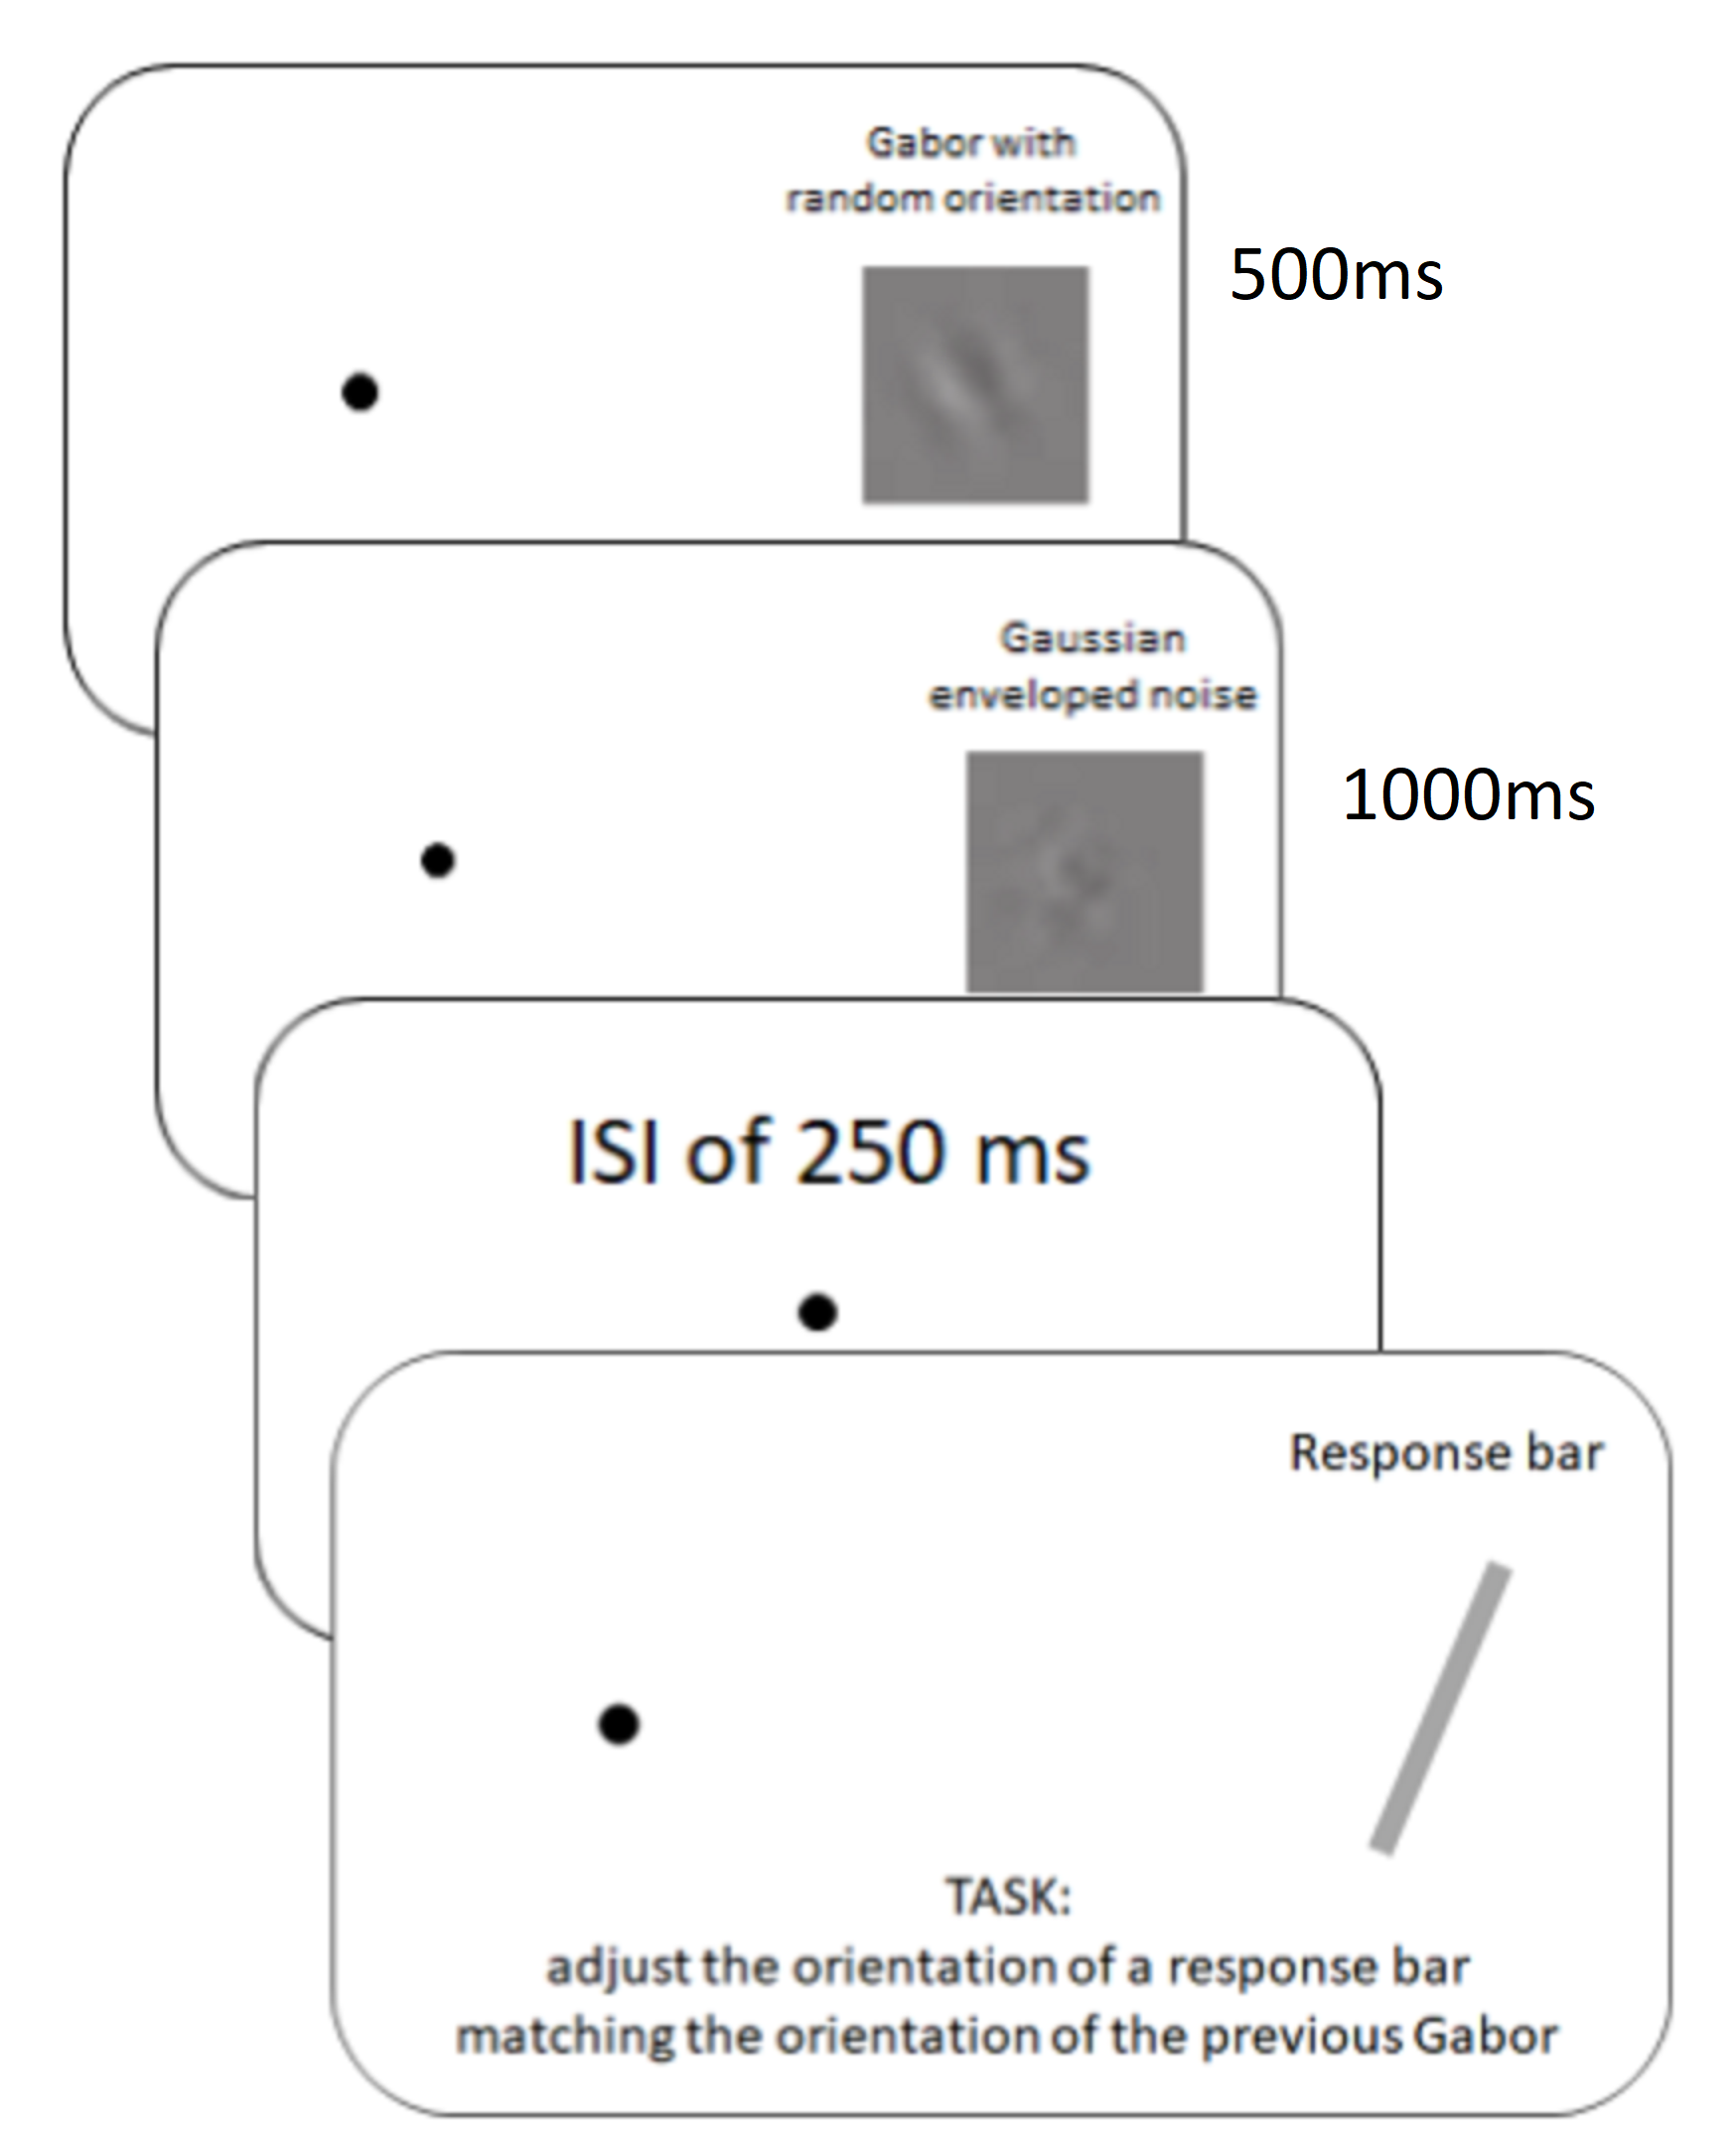
\includegraphics[scale=0.22]{figures/methods/Experimental Task.png}
    \caption{Stimulus time-course. Participants were asked to fixate on the dot, and stimuli were shown at seven degrees eccentricity in the right visual field. In seventy percent of trials, participants were asked to orient a response bar to match the stimulus Gabor patch target.}
    \label{stim_course}
\end{figure}

\subsection*{MEG Analysis}
\subsubsection*{Preprocessing}
MEG data was preprocessed in Python with the MNE-Python package \citep{mne}. Analysis was performed on 204 planar gradiometers (the 102 magnetometers were not used for analysis). Trials were epoched from the onset of a Gabor patch stimulus to 375 milliseconds after the stimulus onset, with 16 time points for each epoch, separated 25 ms apart. An MEG epoch is represented as 204 x 16 data matrix, where each of the 204 rows represents the MEG data for a single gradiometer for a particular behavioral trial, and each column represents the MEG data for all gradiometers at a 25ms time step after stimulus onset. Epochs were rejected for a subject if maximum peaks for any gradiometer exceeded a threshold of $4000\times10^{-13}  \frac{T}{m}$. MEG data was band-pass filtered from 2-40hz, removing any potential low-frequency artifacts and unused high-frequency data. Independent component analysis (ICA) was conducted for each subject to remove artifacts caused by ECG and EOG artifacts. ICA performs source separation for statistically independent components of signals. The top eighty independent components were visually inspected for each subject, and independent components resembling ECG and EOG artifacts were excluded from the filtered MEG dataset. An example of these components is seen in figure \ref{ica_exclude}. Here, we see that the left component represents artifacts resulting from eye blinks (EOG), while the right component represents ECG artifacts.  Six hundred to eight hundred epochs were analyzed for each subject.

\begin{figure}
    \centering
    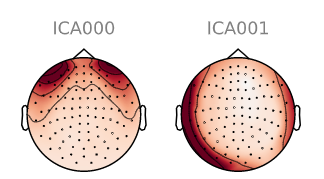
\includegraphics{figures/methods/ica_figure.PNG}
    \caption{Example ICA Components to be excluded. Left: EOG artifact, Right: ECG artifact}
    \label{ica_exclude}
\end{figure}

\begin{figure}
    \centering
    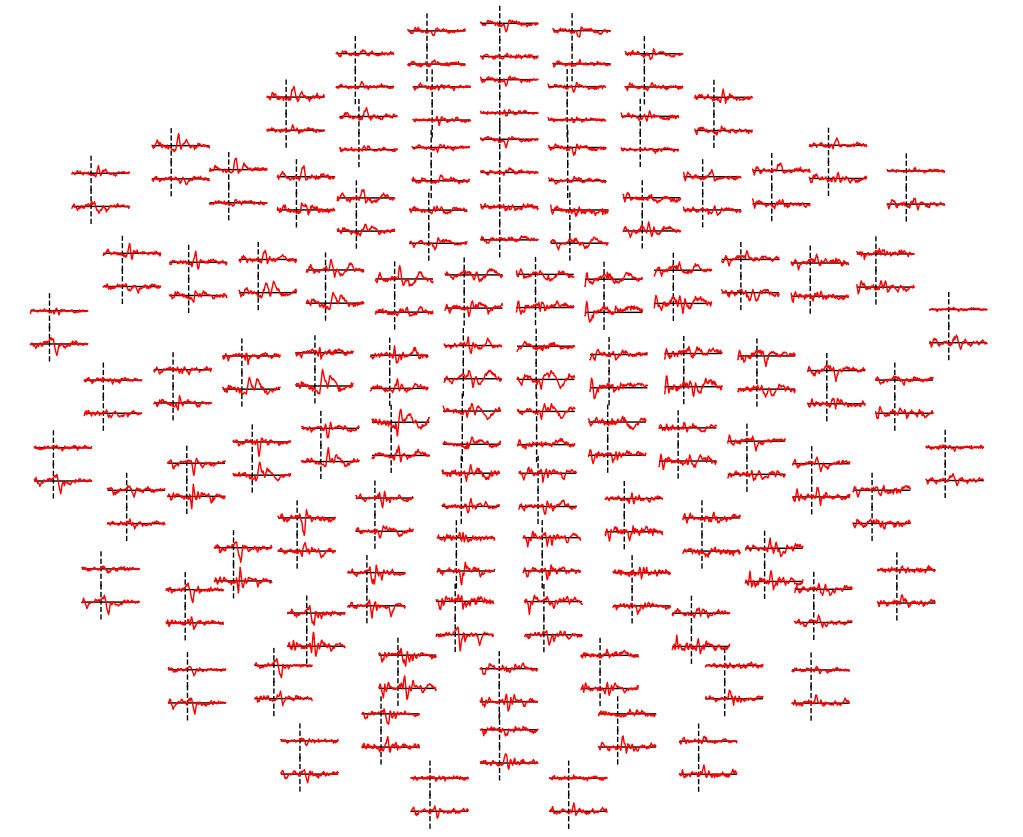
\includegraphics[scale=0.6]{figures/methods/good_topomap.PNG}
    \caption{Example of a representative ERF for a subject}
    \label{good_topomap}
\end{figure}

\subsubsection*{ERF Analysis}
The averaged evoked responses for each subject were measured to ensure that visual responses
appeared in the occipital area as expected. Time-locked epoch responses were averaged over all
trial blocks for each subject at each electrode and visually analyzed for aberrations. In a typical subject, shown in Figure \ref{good_topomap}, evoked responses were observed in left occipital and temporal electrodes around 0.2 seconds after the stimulus was presented. Because the stimulus was only shown in the right visual field, there was limited activation in the right hemisphere.

\subsection*{Source Localization Analysis}
In source localization analysis, we estimated an inverse solution, i.e. the sources of underlying neural activations underlying the MEG sensor readings \citep{mne}. The goal was to convert from sensor space, or the readings at MEG electrodes, to source space, or the estimated activations on the cortical surface. To generate a source localization estimate of our MEG data, we followed the basic process outlined by MNE-Python \citep{mne}. This first required pre-processing the MRI data for each subject. We first computed the cortical surface reconstruction from each subject's anatomical MR image using FreeSurfer's recon-all function \citep{DALE1999179}. We then used the skull stripping approach \citep{segonne_2004} implemented in FreeSurfer as mri watershed. Next, we performed co-registration with our MRI and MEG data, lining up the MEG sensors with the reconstructed MR image according to fiducial markers on the scalp. This aligns the coordinate systems of the MEG space and MRI space. Finally, we performed the MRI watershed procedure again in the new coordinate system.

We next computed a solution to the forward problem for each subject. The forward problem involves computing the external magnetic field at various sensor locations on the scalp resulting from primary currents \citep{mosher99}. MEG electrodes read both primary and secondary currents; primary currents represent microscopic cellular currents that are associated with cognitive processes, while secondary currents are associated with macroscopic electric fields that we are less interested in \citep{mosher99}. To solve the forward problem, we first computed the source space locations for each subject, i.e. the locations of elementary dipole sources that we computed the forward operator at \citep{mne}. Each dipole is analogous to a sensor location located on the cortical surface. To compute these locations, we inflated each cortical surface into a sphere, and overlaid an octahedron onto it. We then subdivided this octahedron 6 times (oct6), giving us 4098 dipole locations for each hemisphere \citep{mne}. We then calculated the Boundary Element Method (BEM) solution with MNE-python using the linear collocation algorithm \citep{mosher99, hamalainen89} for each subject. Using the BEM solution, source space, and the evoked response for a subject, we computed the forward solution as implemented in MNE-python.

Once the forward solution was calculated, we were able to estimate the inverse solution with MNE \citep{mne}. We first used a weighted minimum norm estimate \citep{fuchs_1999, lin_2006} with a loose orientation approach \citep{lin_2005} to estimate source current densities. This approach used our forward solution and the covariance matrix from our epoched data. Source estimates were then computed from the source current densities using dynamic statistical parameter mapping (dSPM) \citep{DALE200055}. These source estimates contained source amplitudes epoched at stimulus onset for each of the 4098 sources in each hemisphere at 16 timesteps, and could then be incorporated into a decoding pipeline as numpy arrays. An example source estimate can be seen in Figure \ref{source_ka}. To validate the results of our source localization estimates of the inverse solution, we plotted the average source space response after stimulus onset for each subject, and compared each source space response to the corresponding sensor space response. We checked that source space responses occurred in the occipital lobe, and ensured that source space peaks occurred at the same time as sensor space peaks.

\begin{figure}
    \centering
    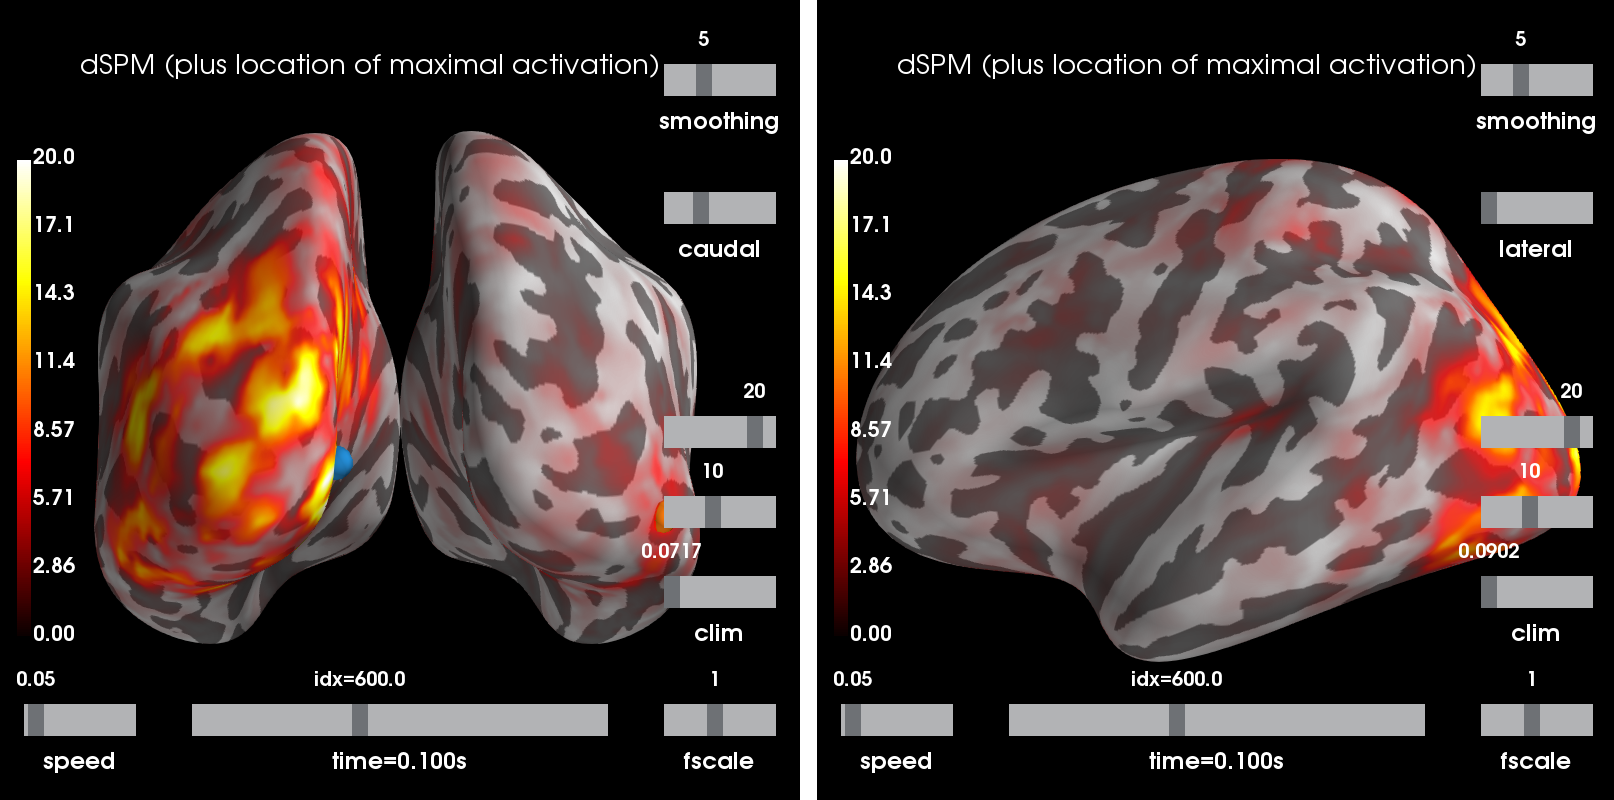
\includegraphics[scale=0.4]{figures/methods/source_loc_KA.png}
    \caption{Average source estimate for subject one subject at 100 ms after stimulus onset. Activations originate in the occipital lobe.}
    \label{source_ka}
\end{figure}

\subsection*{Decoding Stimulus Orientation from MEG Data}
\subsubsection*{Data Processing}
Analysis was performed in Python using decoding libraries from MNE-Python \citep{mne} and the scikit-learn library \citep{scikit-learn}. In the experimental design, Gabor patches were shown at random orientations from 0-180 degrees. For decoding analysis, these Gabor patches were binned into $n$ different classes for decoding model classification. Bins were used because it was difficult to perform a circular regression of orientation angles, especially with relatively few data points. Bin sizes were chosen as a balance between minimizing the angular width of each bin (modeling the original 180 possible Gabor orientations more closely) and maximizing the number of features per bin (giving more trials for each class to improve model performance). Each bin was normalized to have the same number of features by filtering out data points for bins that had more data points than the smallest bin. Decoding models were tested with 4, 8, and 9 bins, and final analysis was performed with 9 bins. Individual models were trained for each subject before calculating group averages to account for individual differences in MEG response.

Gabor patches were binned in bow-tie ranges. These bow-tie ranges put orientations at 0 degrees and 179 degrees in the same orientation bin, as these orientations are nearly identical. For 4 orientation classes, for example, class 0 corresponds to Gabor patches oriented from (0-22.5) degrees and (157.5-180) degrees, class 1 from (22.5-67.5) degrees, class 2 from (67.5-112.5) degrees, class 3 from (112.5-157.5) degrees. If a Gabor patch were to have an orientation of 125 degrees, it would be binned into class 3, and the label of "3" would be used as the classification label in machine learning decoding models. 

For each subject, we originally had 600 or 800 trial epochs. We excluded some trials for each subject to ensure that each orientation bin had the same number of trials, as uneven bin distributions could bias some estimators. Decoding model accuracy was calculated with k-fold cross-validation, where the accuracy metric was the number of correct labels predicted by the model out of the total number of labels predicted. Model accuracy was then compared with the results of a permutation test, in which we shuffled around the training and test labels of the data set to create a null distribution with which to test our null hypothesis. Models were run using both senor space (MEG electrodes) and source space (source estimates) data. There were many more MRI vertices than MEG electrodes, so the weight matrices for the source localization models were much larger than the electrode models. Thus, hyperparameters were tuned differently for the MEG electrode models and source localization models.

The final data had the shape $\mathrm{X} = $ ($n$ epochs $\times$ $m$ sensors/sources $\times$ $t$ time steps) and $\mathrm{y} = $ ($n$ epochs), $1 \leq \mathrm{y}_i \leq 9$, $\mathrm{y}_i \in N$, where X represents the trial epochs for each subject, and y represents corresponding orientation bins for each trial.

\subsubsection*{Permutation Test}
A permutation test was used to determine the statistical significance of the various decoding experiments. Here, features will refer to the $n \times m \times t$ MEG data matrix with $n$ epochs, $m$ electrodes, and $t$ time steps, and the $\omega$ labels refer to the classification bins of the stimulus Gabor orientations, where label $i$ is the label corresponding to the feature data for epoch $i$. In this test, each model was trained 10 times with randomly selected training and test trials to determine the performance of the experimental model. The same analysis was conducted another 100 times with shuffled labels, i.e. the permutation test. In each of these 100 iterations, the labels were shuffled, separately from the corresponding feature vector. This label shuffling removes any structured relationship between features and labels. Thus, these permuted trials will give us a null distribution for our experiment, where the null hypothesis suggests that there is no structured relationship between the MEG features and the labels. To calculate a p-value, the performance of each of the $n = 100$ permutation trials is compared against the $m = 10$ experimental trials, as follows. 
$$\rho = \frac{1}{m}\sum_{i=1}^{m}{\frac{1}{n}\sum_{j=1}^{n}{f(exp_i, perm_j)}}$$
$$f(exp_i, perm_j) = 1 \mbox{ if } perm_j \geq exp_i \mbox{, } 0 \mbox{ otherwise}$$
$$ exp_i = \mbox{ performance of experimental trial } i$$
$$ perm_j = \mbox{performance of permutation trial } j $$

This can be thought of as the proportion of permutation trials that outperform a particular experimental trial, averaged over all of the experimental trials. A low p-value suggests that the experimental trials are on the tail end of the null distribution, suggesting that there may be a structured relationship between the features and labels of the dataset, disputing the null hypothesis.


\subsubsection*{Sliding Logistic Regression Model}
The first machine learning model used was a sliding logistic regression model, which calculated a separate accuracy for each time step of our MEG input signal. For 16 time steps, we calculated 16 different logistic regression weights, and updated these weights using a gradient descent procedure while training. The model was regularized with an elastic net regularization term, which acts as a combination of L1 and L2 regression. This regularization term helped enforce sparsity within our model and prevented weights that were too large, combining the traditional benefits of L1 and L2 regularization. The model also used a "select K best" routine that selected the $K$ best features from the model, based on their contributions to the accuracy. We then tuned the hyperparameters for these additions to our model, namely the size of $K$, the ratio between L1 and L2 loss for elasticnet, and the regularization parameter $C$. The hyperparameters were tuned to get the best cross-validation accuracy.

Here, logistic regression models $\mathrm{Pr}(\textrm{orientation of stimulus } (\mathrm{y}_i) = \omega | \mathrm{X}_i)$. We used multinomial logistic regression for multi-class prediction with logistic regression. The logistic regression model was used for its simplicity and interpretability. The model was relatively easy to implement, especially with the machine learning packages that are already built into scikit-learn \citep{scikit-learn} and mne-python \citep{mne}. The model had only one layer, making it relatively fast to run the model and tune the model parameters. This also meant that we could interpret the weights easily, as there was a one-to-one correspondence between a particular weight and feature from an MEG electrode or MRI vertex. This told us that if a particular weight had a high value, the corresponding electrode/vertex was weighted highly in the model.

\subsubsection*{Sliding Support Vector Machine}
We then implemented a similar sliding SVM model. We again used the scikit-learn \citep{scikit-learn} implementation of the SVM. Our model used relatively high regularization, i.e. a small $C$ parameter in the SVM model, as we found the SVM prone to overfitting. We again used the "select K best" routine to select the $K$ best features in our model. Model weights were updated using a gradient descent procedure. Model accuracy was generated with 5-fold cross-validation. 


\subsubsection*{Inverted Encoding Model}
The final decoding model was the IEM \citep{Brouwer09, Brouwer, GARCIA2013515,sprague_serences_2013, sprague_saproo_serences_2015}. The IEM calculates the predicted responses of each classification channel based on the MEG data, rather than giving a class prediction. This model is well-suited for orientation decoding because it uses a cosine basis set to transform the input data, modeling the inputs better than a linear scale from 0 to 179. In the cosine basis set (shown in Figure \ref{basis_set}a), a perfect channel response centered at 160 degrees would propagate equally to the right and left and wrap around the unit circle, having a similar response at 140 degrees and 180 degrees, and 120 degrees and 20 degrees. This can be seen in Figure \ref{basis_set}b.

\begin{figure}
    \centering
    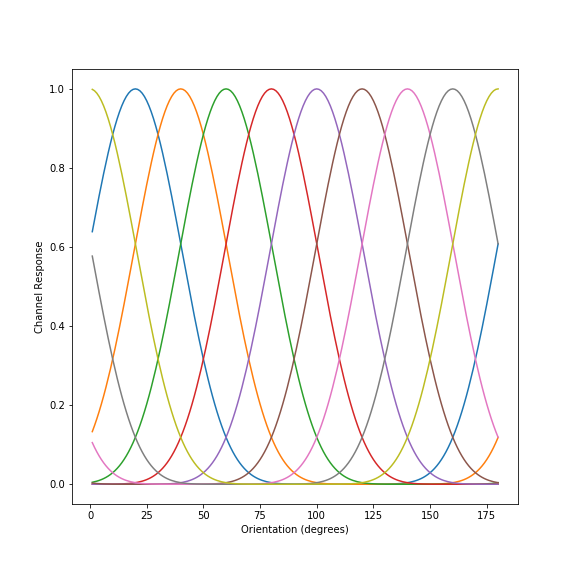
\includegraphics[scale=0.7]{figures/methods/basis_set.png}
    \caption{a) An example cosine basis set for 9 orientation classes. Each color represents the basis function for a single orientation channel, where the cosine function peaks at that orientation channel. b) The ideal channel response for a stimulus oriented at 160 degrees.}
    \label{basis_set}
\end{figure}

To compute the predicted channel response for our MEG data, we first constructed a hypothetical channel response $\mathrm{C}$, a matrix of number of epochs $\times$ number of orientation channels. This was computed by matrix multiplying a stimulus mask matrix by the cosine basis set. The size of the stimulus mask matrix was number of trials $\times$ 180, where row $i$ had value 1 at the degree of trial $i$'s stimulus orientation, and 0 elsewhere. In the problem formulation of the IEM, there was the MEG input data, $\mathrm{B_{train}}$ with shape (number of epochs $\times$ number of MEG electrodes), which was related to the channel response set, $\mathrm{C_{train}}$, by the following formula:
$$ \mathrm{B_{train} = W C_{train}}$$
We first computed $\mathrm{\hat{W} = B_{train} C_{train}^T (C_{train} C_{train}^T)^{-1}}$, the linear least squares estimate for W. We then solved for the predicted channel responses $\mathrm{C_{test}}$  of our test set, related to the test MEG data $\mathrm{B_{test}}$ by the formula $\mathrm{B_{test} = W C_{test}}$, which was estimated by least squares as 
$$\mathrm{C_{test} = (\hat{W}^T \hat{W})^{-1} \hat{W}^T B_{test}}$$

We then performed k-fold cross-validation to generate accuracy over all the trials, and performed this analysis at each time step. The channel response is informative on its own, but we can also generate a classification for a trial by taking the argmax of the channel response (channel corresponding to maximum channel response) for a particular trial.

\subsubsection*{Previous Orientation Decoding}
After decoding the orientation of stimulus $t$ from MEG, we attempted to decode the orientation of the $(t-1)$th stimulus from the MEG response data corresponding to the $t$th trial. If the previous stimulus orientation biases the current stimulus orientation perception, then it's possible that a decoding model could reverse engineer this bias and decode the orientation of the previous stimulus. This analysis was computed with the same decoding models as the current stimulus decoding, but we shifted the data labels backward by one time step in relation to the data, such that the data at time $t$ was used to predict the label at time $t - 1$. We performed the same permutation test as in previous decoding models to test the significance of this previous trial decoding.

\subsection*{Serial Dependence Analysis}

\subsubsection*{Behavioral Analysis}
Before performing decoding analysis for temporal bias (how the previous stimulus affected the decoding of the current stimulus), we performed the serial dependence analysis outlined in \cite{fischer_whitney_2014} to determine if any serial dependence effect existed in our data. For each subject, we calculated the error for a trial (reported orientation - presented orientation), where positive values indicate errors in the clockwise direction. For each trial, we calculated the difference between the previous and current trial for each trial, where a positive value signifies that the previous orientation was more clockwise than the current orientation. We plotted the error on the y-axis and the previous-current trial difference on the x-axis. We then fit the error plot with a derivative of Gaussian (DoG) curve, allowing us to measure the amplitude of the serial dependence effect. This curve is modeled by the function, $y = (a b c) x e^{-(b x)^2}$, where $x$ is the relative orientation of the previous trial, $a$ is the amplitude of the DoG curve, $b$ is the DoG curve width, and
$c = \frac{\sqrt{2}}{e^{-0.5}}$.

Error bars were generated by bootstrapping the DoG curve fit 5000 times, sampling with replacement. To generate $P$ values for this DoG curve, a permutation test was again used, generating 100,000 DoG curves with shuffled data labels (relative previous orientation) for each iteration. The amplitudes of the permuted DoG fits were compared against the measured amplitude of the participant DoG fits, and the $P$ value was taken as the proportion of permuted amplitudes that were greater than or equal to the measured subject amplitude. This analysis was performed using the lmfit library for python \citep{newville_matthew_2014_11813}.



\subsubsection*{Channel Response Bias Analysis}
We next investigated how the relative previous stimulus orientation affected the decoding of the current stimulus. We again calculated the relative previous stimulus orientation (previous orientation - current orientation) for each trial, where positive values indicate that the previous orientation was more clockwise than the current one. We then ran the same k-fold cross-validation decoding process on our MEG data with the IEM. We generated the channel responses for each orientation for each trial. We could then bin these channel responses and class probabilities by relative previous orientation to reveal any relationship between model predictions and relative previous orientation. Each bin was normalized to have the same number of entries. We then centered each channel response such that the actual label of the data lined up with the same label for all trials. For example, if we aligned all responses to channel 5, and trial $i$ had a label of channel 3, we rolled the channel response for $i$ two places to the right. 

We first performed a pixel-wise analysis of channel response bias. We subtracted the mean channel response from all bins, giving us the deviation of each bin from the mean. If there was any impact of serial dependence on decoding, we would expect to see channel response biased away from the mean in certain bins. To test how significantly each bin deviates from the mean, we performed another permutation test, this time shuffling the bin that each channel response falls into. We then calculated a $P$ value for each channel response orientation in each relative previous orientation bin. This P value was calculated as the proportion of permutations that had greater deviation from the mean than the measured channel response for said bin.

We then fit a Gaussian function to each relative previous orientation bin at each time step, as the pixel-wise analysis was not necessarily suited for a more subtle bias structure. We performed a permutation test by shuffling the relative previous orientation bin for each subject. We fit a Gaussian to each shuffled relative previous orientation bin. To generate P values for this analysis, we compared the absolute values of the decoded Gaussian means and the permutation Gaussian means.

\end{document}